\chapter{方法}

\label{sec:method}
本节首先在 \S\ref{preliminary} 中回顾 VLA 的核心算法原理，它构成了对抗方案设计的基础。随后，我们介绍两类非目标对抗攻击，包括 \S\ref{Normalized_Action_Discrepancy_Attack} 中的非目标动作差异攻击（Untargeted Action Discrepancy Attack, UADA）以及 \S\ref{Geometry_aware_Attack} 中的非目标位置感知攻击（Untargeted Position-aware Attack, UPA）。在 \S\ref{Target_Attack} 中，我们进一步提出目标操控攻击（Targeted Manipulation Attack, TMA），其目标是诱导机器人朝特定错误执行方向运动。最后，我们在 \S\ref{NAD_metric} 中引入归一化动作差异（Normalized Action Discrepancy, NAD）指标。整体框架如图~\ref{fig:main} 所示。

\section{预备知识} \label{preliminary}
\textbf{视觉-语言-动作模型}~\cite{Brianna2023RT2,kim24openvla}（见图~\ref{fig:main}）建立在集成视觉编码器的大语言模型之上，使机器人能够理解人类指令并处理来自摄像头的视觉输入，从而执行具备上下文感知能力的动作。VLA 模型~\cite{kim24openvla,Brianna2023RT2,Li2024LLaRA}通常通过对机器人动作进行离散化，将连续动作预测抽象为分类问题。具体来说，它们首先将连续概率离散为类别标签 $y = \arg \max \mathcal{F}(x)$，其中 $\mathcal{F}(\cdot)$ 为 VLA 模型。随后，动作去标记器生成动作 $A=DT(y)$。
通过将动作值划分为离散类别标签，模型把连续概率输出转化为离散信号。这种简化有助于更快收敛并加快训练速度，因此在基于 VLA 的模型中被广泛采用~\cite{kim24openvla,Brianna2023RT2,Li2024LLaRA}。

本文关注一个具有 7 个自由度（DoFs）的机械臂~\cite{haddadin2022franka}。在每个时间步，动作由 7 个在三维笛卡尔空间中具有明确物理意义的自由度构成，可表示为：
\begin{equation}
    A=[\Delta{P_x}, \Delta{P_y}, \Delta{P_z}, \Delta{R_x}, \Delta{R_y}, \Delta{R_z}, \text{gripper}],
\end{equation}
其中 $\Delta{P_{x,y,z}}$ 和 $\Delta{R_{x,y,z}}$ 分别表示沿 x、y、z 轴的相对位置变化和旋转变化，并在各个自由度的动作边界 $[y_{\min}^i,y_{\max}^i]$ 上被离散为 256 个均匀 bin~\cite{kim24openvla}。$gripper$ 状态是二值的，表示夹爪张开或闭合。该控制设计为对抗攻击带来了独特挑战，因为精细划分的 bin 会使相邻 bin 之间的动作差异极小（例如 $\pm$0.007/bin）。这意味着，即便攻击仅将分类结果推移到相邻 bin，所产生的动作偏差对真实世界性能的影响也非常有限。

\section{非目标动作差异攻击} \label{Normalized_Action_Discrepancy_Attack}
为了加剧动作偏差，我们提出非目标动作差异攻击（UADA），其目标是最大化机器人动作中的偏离程度。
这一攻击建立在如下观察之上：更大的机器人动作通常对应更强烈的物理运动，而这又可能放大真实世界中的潜在危险~\cite{iso_10218,iso_15066,ISO13482}。
对于 UADA，攻击目标是 7 个自由度中的单个自由度或其组合，记为 $y^I_{gt}=\{y^{i}_{gt}|i\in[1,\dots,7]\}$。
为了定义 UADA 的目标函数，我们首先确定最远动作 $y_{adv}^i$，它能够使第 $i$ 个自由度相对于真实动作 $y^i$ 的偏差达到最大。对于每个自由度，该动作对应其动作边界 $[y_{\min}^i,y_{\max}^i]$ 中距离真实动作更远的一端，形式化定义为：
\begin{equation}
y_{adv}^i =
\begin{cases} 
y_{\max}^i, & \text{if } |y_{\max}^i-y^i_{gt}| \geq |y_{\min}^i-y^i_{gt}| \\
y_{\min}^i, & \text{otherwise}
\end{cases}.
\end{equation}
我们并不直接将 $y_{adv}^i$ 作为误分类目标，而是引入一个软攻击目标来刻画动作之间的差异，从而保证梯度优化更平滑、攻击表现更稳定。具体而言，由于 bin 标签本身包含物理动作幅值信息，我们使用归一化 bin 标签 $y^i_{bins}=[\frac{1}{bins},\dots,1]$ 对输出概率 $\mathcal{F}(x)^i_{bins}\in\mathcal{R}^{_{1\times{bins}}}$ 进行重加权，其中 $\lfloor y^i_{bins} \rfloor$ 与 $\lceil y^i_{bins} \rceil$ 分别对应 $y_{\min}^i$ 和 $y_{\max}^i$ 的归一化值。重加权过程定义为：
\begin{equation}
    y_{soft}^{i}= \sum_{bins=1}^{n}  \mathcal{F}(x+\delta)^i_{bins} \otimes y^i_{bins},
\end{equation}
其中 $\otimes$ 表示 Hadamard 积，$\delta$ 为对抗补丁，$y_{soft}^{i}$ 表示第 $i$ 个自由度的软动作。最终，UADA 的目标是最小化软动作与最远动作之间的差异，即：
\begin{equation}
    \mathcal{L}_{\text{UADA}} = \mathbb{E}_{(x,y)\sim\mathcal{X}}\sum_{i}^{I} (y_{soft}^{i}-y_{adv}^i)^2,
\end{equation}
UADA 定义了一个专门针对机器人动作空间的目标函数 $\mathcal{L}_{\text{UADA}}$，使对抗补丁能够在任务表现上制造显著且持续的干扰。

\section{非目标位置感知攻击} \label{Geometry_aware_Attack}
我们进一步从位置动力学的角度并行探索 VLA 模型中的非目标对抗攻击。在典型任务执行过程中，末端执行器必须朝指定目标进行精确且定向的移动，而这些动作映射在三维空间中。位置相关自由度 $A^p = [\Delta{P_x}, \Delta{P_y}, \Delta{P_z}]$ 则概括了在三维空间中实现有效机器人控制所需的方向性移动。

考虑到 $A^p=DT(y^{p})$ 对控制末端执行器路径的重要性，我们提出一种位置感知攻击，用于破坏原本预期的运动轨迹。这类对抗脆弱性尚未被充分研究，但对任务失败具有重要影响：该攻击目标通过引入方向扰动，使末端执行器偏离预期路径，进而放大误差并造成明显的轨迹扭曲。形式化地，我们将非目标位置感知攻击（UPA）目标定义为：

\begin{equation}
    \mathcal{L}_\text{UPA}= \mathbb{E}_{(x,y)\sim\mathcal{X}}\big[\alpha\frac{y^{p}_{adv} \cdot y^{p}}{\|y^{p}_{adv}\| \|y^{p}\|}+\beta\frac{1}{||y^{p}_{adv}-y^{p}||_2}\big],
    \label{eq:gaattack}
\end{equation}
% \begin{equation}
%     \textcolor{red}{
%     \mathcal{L}_G= \mathbb{E}_{(x,y)\sim\mathcal{X}}\big[\mathcal{L}_{cos}(y^{pos}_{adv},y^{pos}_{gt})+\mathcal{L}_2(y^{pos}_{adv},y^{pos}_{gt})^{-1}\big]
%     }
% \end{equation}
其中 $\alpha$ 和 $\beta$ 为平衡扰动方向性与幅度的超参数。通过将几何感知引入攻击过程，该方法即便只进行很小的调整，也能生成会在机器人轨迹中累积偏离的扰动。进一步的 $L_2$ 归一化 $||\cdot||_2$ 会强化这些偏移，使攻击具有很强的有效性和破坏性。

\begin{figure}[!h]
    \centering
    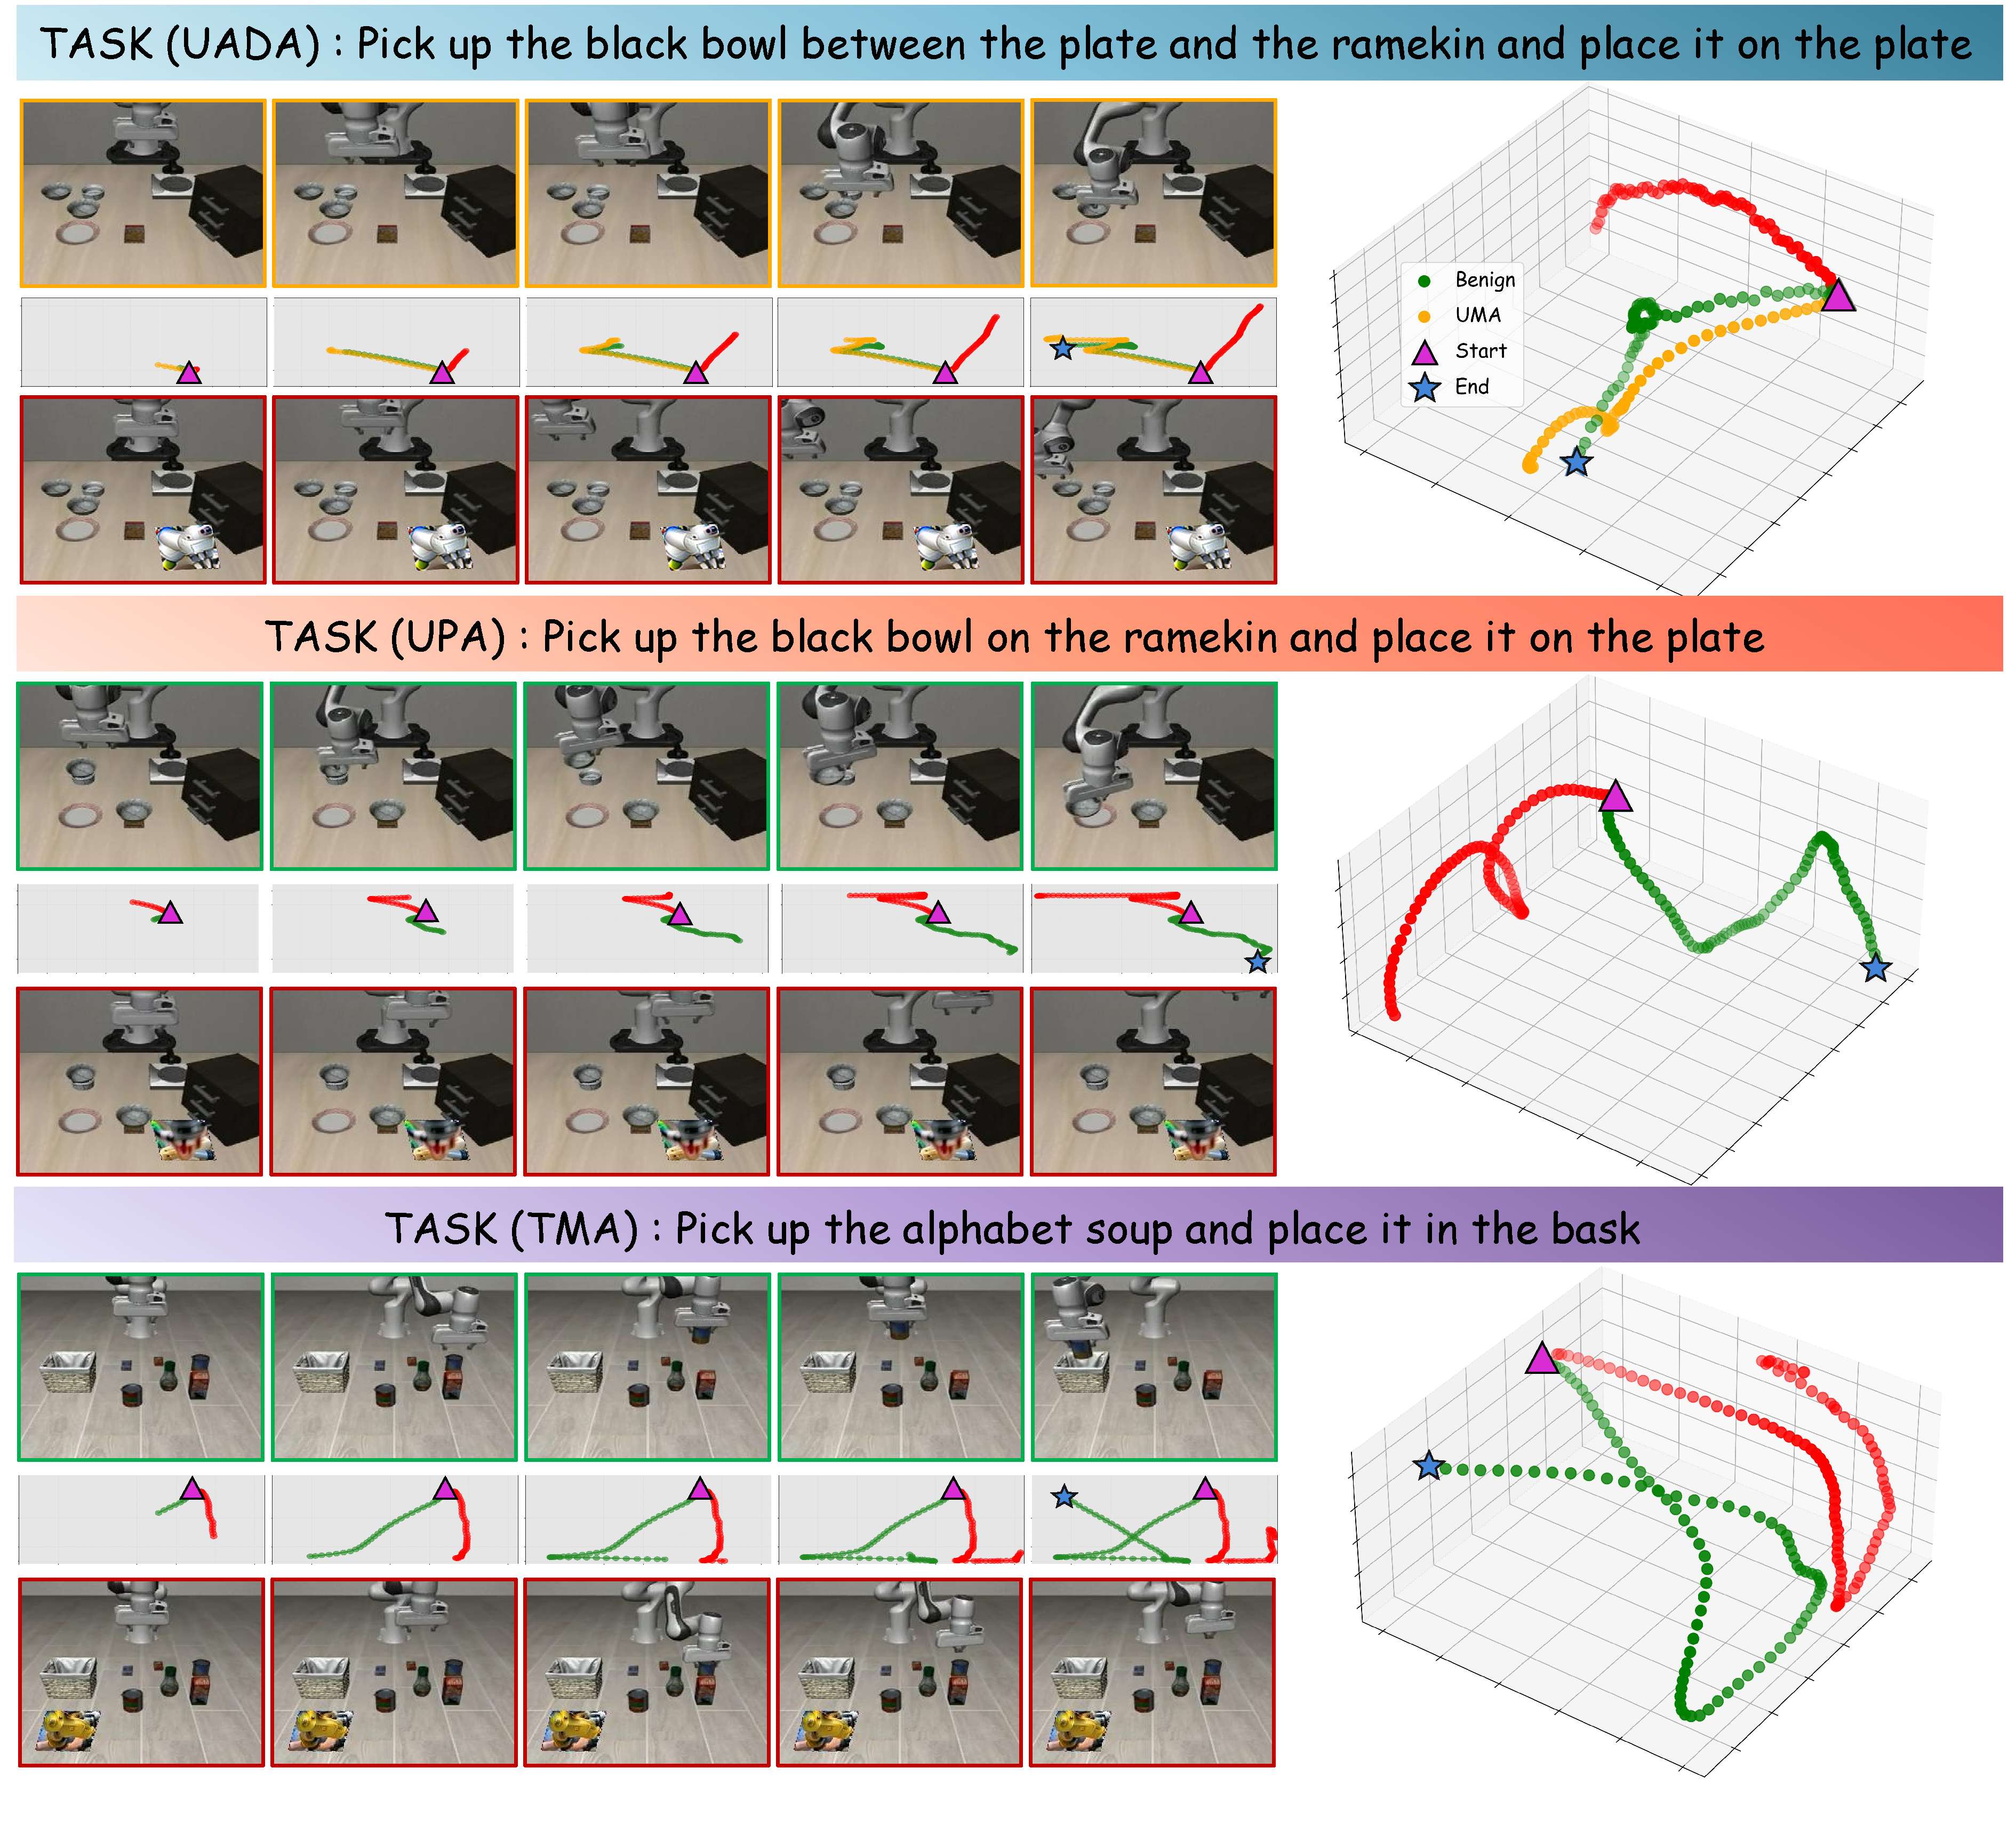
\includegraphics[width=0.84\linewidth]{images/vis3.pdf}
    \vspace{-1.7em}
    \caption{在 OpenVLA-7B~\cite{kim24openvla} 和 OpenVLA-7B-LIBERO~\cite{kim24openvla} 上，采用 \textcolor[HTML]{3A7F9A}{UADA}、\textcolor[HTML]{FF6F59}{UPA} 和 \textcolor[HTML]{7A5C9E}{TMA} 三种目标时的\textbf{定性结果}。我们在每个时间步可视化良性场景 \textcolor[HTML]{218F20}{$\bullet$} 与对抗场景 \textcolor[HTML]{FB0C0F}{$\bullet$} 的整体 3D 轨迹和 2D 轨迹，以比较所生成对抗补丁对其造成的影响。在 UADA 任务中，还可视化了非目标轨迹 \textcolor[HTML]{FDB117}{$\bullet$}。所有轨迹均以 \textcolor[HTML]{dc2cd4}{\ding{115}} 为起点，成功终点以 \textcolor[HTML]{3A7F99}{\ding{72}} 标记。}
    \label{fig:qualitative}
    \vspace{-1.5em}
\end{figure}

\section{目标操控攻击}\label{Target_Attack}
除上述非目标攻击外，我们还采用目标策略来探索 VLA 模型的对抗脆弱性。
该攻击旨在直接误导模型预测特定轨迹，从而产生精确的动作修改。我们之所以设计这一攻击，是因为目标化修改能够驱动恶意行为或诱发任务失败。目标操控攻击的目标函数为：
\begin{equation}
\mathcal{L_\text{TMA}}=\mathbb{E}_{(x,y)\sim\mathcal{X}}[CE(\mathcal{F}(x + \delta)^I, y^I_T)],
\label{eq_tma}
\end{equation}
其中 $ y^I_T=\{y^{i}_T=t|i\in[1,\dots,7],t\in [y^i_{\min},y^i_{\max}]\}$ 表示对抗目标；$CE(\cdot,\cdot)$ 表示交叉熵损失，用于衡量在对抗扰动下预测状态与目标状态之间的误差。通过在连续时间步中将机器人引向对抗目标，我们的方法能够操纵轨迹并削弱任务表现，最终对预期操作造成显著破坏。
此外，无论操纵单个自由度还是多个自由度的组合，都可能严重破坏任务成功率，因为某一维度上的误差往往会在执行过程中不断传播并随时间放大（见图~\ref{fig:qualitative}）。

\section{指标：归一化动作差异} \label{NAD_metric}
为了评估对抗补丁可能造成的物理影响，我们提出归一化动作差异（NAD）作为一个用于评估动作层面偏差的细粒度指标。NAD 作为任务层面粗粒度失败率（Failure Rate, FR）的补充度量，能够对动作执行过程中的偏移进行更细致分析。为定义 NAD，我们首先确定最大动作差异 $d^i_{\text{max}}$，它表示第 $i$ 个自由度在允许范围内可能出现的最大偏移。该值通过计算真实动作 $y^i_{gt}$ 与其动作边界 $[y^i_{\min},y^i_{\max}]$ 之间的 L1 距离得到：
\begin{equation}
    d_{\text{max}}^i (y) = \max \big[DT(| y^i_{gt} - y^i_{\min} |), DT(|y^i_{gt} - y^i_{\max} |)\big].
\end{equation}
接着，我们计算实际动作差异 $d_{\text{applied}}^i(x,y)$ $=|DT(\mathcal{F}(x)^i)-DT(y^i_{gt})|$，用于衡量模型输出与真实动作之间的偏移。
我们将 NAD 定义为 $d_{\text{applied}}^i$ 与 $d_{\text{max}}^i$ 的偏移比值：
\begin{equation}
    \rm{NAD} = \frac{1}{I}\sum_i^I \frac{d^i_{\text{applied}}}{d^i_{\text{max}}},
    \label{formula:AD}
\end{equation}
其中 $I\in[1,\dots,7]$ 表示单个自由度或多个自由度的组合。通过这一方式，NAD 为动作偏差提供了归一化度量，使得我们能够在不同自由度设置下对对抗影响进行一致评估。
